\chapter{Analisis}
\label{chap:analisis}

Pada bab ini akan dibahas analisis terhadap teori-teori yang telah dibahas sebelumnya. Analisis akan meliputi studi kasus untuk algoritma \textit{secret sharing} shamir yang telah dibahas sebelumnya, algoritma \textit{secret sharing} shamir yang dikembangkan, dan perancangan perangkat lunak.

\section{Studi Kasus}
Bagian ini akan berisi studi kasus mengenai algoritma \textit{secret sharing} shamir yang telah dibahas sebelumnya dan algoritma \textit{secret sharing} shamir yang telah dikembangkan.

\subsection{\textit{Secret Sharing} Shamir}
Pada bagian ini akan dijelaskan proses pembangunan \textit{share} untuk \textit{secret sharing} shamir pada sebuah data \textit{S}, proses pembangunan kembali \begin{math}S\end{math} dari \textit{share-share} yang ada, dan proses penyelesaian persamaan linear untuk pembangunan kembali \begin{math}S\end{math}. Untuk contoh kasus ini, diasumsikan jenis data yang digunakan adalah angka positif, dipilih \begin{math}S=1234\end{math}.

\begin{flushleft}
	\textbf{Proses pembangunan \textit{share}}
\end{flushleft}

Langkah yang perlu dilakukan pertama adalah memilih banyak \textit{share} \begin{math}n\end{math} yang diinginkan dan banyak minimal \textit{share} yang diperlukan untuk mengembalikan \begin{math}S\end{math}, yaitu \begin{math}k\end{math}. Untuk kasus ini, akan dipilih \begin{math}n=8\end{math} dan \begin{math}k=3\end{math}.

Langkah selanjutnya adalah memilih \begin{math}k-1\end{math} angka acak yang nanti akan digunakan sebagai koefesien fungsi polinomial \begin{math}f(x)\end{math}. Karena pada kasus ini \begin{math}k=3\end{math} maka ada 2 angka acak yang dipilih, misalkan 237 dan 55. Maka fungsi \begin{math}f(x)\end{math} untuk menghitung nilai setiap \textit{share}:

\begin{displaymath}
	f(x) = 1234 + 237x + 55x^2
\end{displaymath}

Kemudian, akan dihitung nilai dari setiap \begin{math}f(x_i)\end{math} dari \begin{math}f(1)\end{math} sampai \begin{math}f(8)\end{math} karena \begin{math}n=8\end{math}:

\begin{gather*}
	f(1) = 1234 + 237*1 + 55*1*1 = 1526	\\
	f(2) = 1234 + 237*2 + 55*2*2 = 1928	\\
	f(3) = 1234 + 237*3 + 55*3*3 = 2440	\\
	f(4) = 1234 + 237*4 + 55*4*4 = 3062	\\
	f(5) = 1234 + 237*5 + 55*5*5 = 3794	\\
	f(6) = 1234 + 237*6 + 55*6*6 = 4636	\\
	f(7) = 1234 + 237*7 + 55*7*7 = 5588	\\
	f(8) = 1234 + 237*8 + 55*8*8 = 6650
\end{gather}

Maka diperoleh nilai untuk setiap \begin{math}S_1\end{math} sampai \begin{math}S_8\end{math}.
\begin{displaymath}
	S_1 = 1526, S_2 = 1928, S_3 = 2440, S_4 = 3062, S_5 = 3794, S_6 = 4636, S_7 = 5588, S_8 = 6650
\end{displaymath}

\begin{flushleft}
	\textbf{Proses pembangunan kembali (rekonstruksi \textit{S})}
\end{flushleft}

Karena pada kasus ini \begin{math}k=3\end{math} maka untuk mengembalikan \begin{math}S\end{math} maka hanya dibutuhkan 3 \textit{share} saja. Misalkan \textit{share} yang dipilih adalah \begin{math}S_2\end{math}, \begin{math}S_4\end{math}, dan \begin{math}S_5\end{math}.

Langkah selanjutnya adalah membentuk rumus dasar dari fungsi \begin{math}f(x)\end{math}. Karena pada kasus ini, \begin{math}k=3\end{math}, maka rumus dasar dari \begin{math}f(x)\end{math}:
\begin{displaymath}
	f(x) = c + bx + ax^2
\end{displaymath}

Setelah rumus dasar dari fungsi \begin{math}f(x)\end{math} dibentuk, langkah selanjutnya adalah menghitung nilai masing-masing fungsi berdasarkan \textit{share} yang diketahui, dalam kasus ini adalah \begin{math}S_2\end{math}, \begin{math}S_4\end{math}, dan \begin{math}S_5\end{math}, maka nilai masing-masing fungsi \begin{math}f(x)\end{math}:
\begin{gather*}
	f(2) = c + 2b + 4a = 1928	\\
	f(4) = c + 2b + 16a = 3062	\\
	f(5) = c + 5b + 25a = 3794
\end{gather}

Langkah selanjutnya adalah menyelesaikan persamaan linear di atas, sehingga nanti bisa diperoleh nilai \begin{math}c\end{math} dimana seperti yang diketahui nilai \begin{math}c\end{math} merupakan \begin{math}S\end{math} karena \begin{math}S\end{math} adalah konstanta tanpa koefesien dari \begin{math}f(x)\end{math} (\begin{math}f(0) = c\end{math}).

\begin{flushleft}
	\textbf{Proses penyelesaian persamaan linear untuk pembangunan kembali (rekonstruksi \textit{S})}
\end{flushleft}

Pada bagian ini akan dijelaskan proses penyelesaian persamaan linear menggunakan eliminasi gauss. Pada kasus ini, persamaan linear yang diperoleh:
\begin{gather*}
	c + 2b + 4a = 1928	\\
	c + 2b + 16a = 3062	\\
	c + 5b + 25a = 3794
\end{gather}

Langkah awal yang perlu dilakukan dalam eliminasi gauss adalah transformasi persamaan linear ke matriks. Maka, dari persamaan linear di atas matriksnya:

\begin{center}
	\setlength\arraycolsep{15pt}
	\[
	\begin{bmatrix}
			1 & 	2 & 	4  & 	1928 \\[1em]
			1 & 	4 & 	16 & 	3062 \\[1em]
			1 & 	5 & 	25 & 	3794
	\end{bmatrix}
	\]
\end{center}

Langkah selanjutnya adalah proses yang dinamakan operasi baris, yaitu operasi aritmatika (tambah, kurang, kali dan bagi) pada setiap baris dari matriks. Proses ini dilakukan sampai diperoleh bentuk matriks segitiga atas, yaitu matriks bujur sangkar yang semua elemen di bawah diagonal utamanya 0. Berikut langkah-langkah proses untuk memperoleh matriks segitiga atas. Sebelumnya, untuk akan diberi label untuk masing-masing baris, baris pertama, \begin{math}L_1\end{math}, baris kedua, \begin{math}L_2\end{math}, dan baris ketiga, \begin{math}L_3\end{math}.

Langkah pertama dari operasi baris untuk membangun matriks segitiga atas adalah mengurangi \begin{math}L_2\end{math} dan \begin{math}L_3\end{math} dengan \begin{math}L_1\end{math} agar setiap elemen kolom pertama di bawah \begin{math}L_1\end{math} nilainya menjadi 0 (nol).

\begin{center}
	\begin{gather*}
		L_2 - L_1	\\
		L_3 - L_1
	\end{gather}
\end{center}

\begin{flushleft}
	Maka, matriksnya menjadi
\end{flushleft}

\begin{center}
	\setlength\arraycolsep{15pt}
	\[
	\begin{bmatrix}
			1 & 	2 & 	4  & 	1928 \\[1em]
			0 & 	2 & 	12 & 	1134 \\[1em]
			0 & 	3 & 	21 & 	1866
	\end{bmatrix}
	\]
\end{center}

\begin{flushleft}
	Kemudian, untuk \begin{math}L_2\end{math} dan \begin{math}L_3\end{math} akan disederhanakan nilainya, dengan cara membagi \begin{math}L_2\end{math} dengan 2 dan \begin{math}L_3\end{math} dengan 3.
\end{flushleft}

\begin{center}
	\begin{gather*}
		\frac{1}{2}L_2	\\
		\frac{1}{3}L_3
	\end{gather}
\end{center}

\begin{flushleft}
	Maka, matriksnya menjadi
\end{flushleft}

\begin{center}
	\setlength\arraycolsep{15pt}
	\[
	\begin{bmatrix}
			1 & 	2 & 	4  & 	1928 	\\[1em]
			0 & 	1 & 	6 & 	567 	\\[1em]
			0 & 	1 & 	7 & 	622
	\end{bmatrix}
	\]
\end{center}

\begin{flushleft}
	Kemudian, \begin{math}L_3\end{math} akan dikurangi oleh \begin{math}L_2\end{math} sehingga, bisa diperoleh matriks segitiga atas.
\end{flushleft}

\begin{center}
	\begin{displaymath}
		L_3 - L_2
	\end{displaymath}
\end{center}

\begin{flushleft}
	Maka, matriksnya menjadi
\end{flushleft}

\begin{center}
	\setlength\arraycolsep{15pt}
	\[
	\begin{bmatrix}
			1 & 	2 & 	4  & 	1928 	\\[1em]
			0 & 	1 & 	6 & 	567 	\\[1em]
			0 & 	0 & 	1 & 	55
	\end{bmatrix}
	\]
\end{center}

Langkah selanjutnya adalah menghitung nilai konstanta untuk masing-masing koefesien dengan cara melakukan substitusi balik. Setiap koefesien pada persamaan diasosiasikan dengan kolom pada matriks, kolom pertama untuk \begin{math}c\end{math}, kolom kedua untuk \begin{math}b\end{math}, dan kolom ketiga untuk \begin{math}a\end{math}. Maka, dari substitusi balik ini diperoleh:

Untuk nilai \begin{math}a\end{math} diperoleh dari \begin{math}L_3\end{math}.
\begin{center}
	\begin{gather*}
		a = 55
	\end{gather}
\end{center}

\begin{flushleft}
	Kemudian, untuk nilai \begin{math}b\end{math} diperoleh dari \begin{math}L_2\end{math} dengan mensubstitusi nilai \begin{math}a\end{math}.
\end{flushleft}

\begin{center}
	\begin{gather*}
		b + 6a = 567 \\
		b + 6*55 = 567 \\
		b = 567 - 330 \\
		b = 237
	\end{gather}
\end{center}

\begin{flushleft}
	Substitusi balik terakhir adalah untuk mendapatkan nilai \begin{math}c\end{math} dengan mensubstitusi nilai \begin{math}a\end{math} dan \begin{math}b\end{math} pada \begin{math}L_1\end{math}, dimana nilai \begin{math}c\end{math} adalah \begin{math}S\end{math} karena seperti yang diketahui, \begin{math}S\end{math} adalah konstanta bebas.
\end{flushleft}

\begin{center}
	\begin{gather*}
		c + 2b + 4a = 1928 \\
		c + 2*237 + 4*55 = 1925 \\
		c = 1928 - 474 - 220 \\
		c = 1234
	\end{gather}
\end{center}

\subsection{Pengembangan Algoritma \textit{Secret Sharing} Shamir}

Jika pada contoh kasus sebelumnya adalah algoritma \textit{secret sharing} shamir pada jenis data angka. Pada bagian ini akan dijelaskan pengembangan dari algoritma \textit{secret sharing} shamir untuk jenis data tulisan atau kalimat. Sama seperti contoh kasus sebelumnya, pada bagian ini ada 3 proses, yaitu proses pembangunan pembangunan \textit{share} untuk data \begin{math}S\end{math}, proses rekonstruksi \begin{math}S\end{math} dari \textit{share-share}, dan proses penyelesaian persamaan linear untuk mengembalikan nilai \begin{math}S\end{math}. Untuk contoh kasus ini, data \begin{math}S\end{math} bentuknya berupa tulisan atau kalimat.

\begin{displaymath}
	S = \text{\textbf{\textit{secret}}}
\end{displaymath}

\begin{flushleft}
	\textbf{Proses pembangunan \textit{share}}
\end{flushleft}

Langkah yang perlu dilakukan pertama adalah memilih banyak \textit{share} \begin{math}n\end{math} yang diinginkan dan banyak minimal \textit{share} yang diperlukan untuk mengembalikan \begin{math}S\end{math}, yaitu \begin{math}k\end{math}. Untuk kasus ini, akan dipilih \begin{math}n=8\end{math} dan \begin{math}k=4\end{math}.

Karena \begin{math}S\end{math} merupakan tulisan atau kalimat, sebelum menentukan angka acak untuk konstanta setiap koefesien, setiap karakter dari \begin{math}S\end{math} (termasuk spasi) harus diubah menjadi angka berdasarkan nilai ASCII. Jadi, untuk masing-masing karakter dalam \begin{math}S\end{math}.

\begin{align*}
	's' &= 115 \\
	'e' &= 101 \\
	'c' &= 99 \\
	'r' &= 114 \\
	'e' &= 101 \\
	't' &= 116
\end{align}

Langkah berikutnya adalah memilih \begin{math}k-1\end{math} angka acak yang nanti akan digunakan sebagai koefesien fungsi polinomial \begin{math}f(x)\end{math}. Karena \begin{math}S\end{math} merupakan tulisan atau kalimat, maka perlu dipilih angka acak untuk setiap karakter dari \begin{math}S\end{math}. Dalam contoh kasus ini, ada \begin{math}k-1\end{math} angka acak untuk masing-masing karakter dari \begin{math}S\end{math} dan karena \begin{math}k=4\end{math}, maka untuk masing-masing karakter terdapat 3 angka acak.
\begin{itemize}
	\item \begin{math}'s'\end{math}: 43, 45, dan 27
	\item \begin{math}'e'\end{math}: 24, 88, dan 54
	\item \begin{math}'c'\end{math}: 48, 31, dan 26
	\item \begin{math}'r'\end{math}: 19, 59, dan 60
	\item \begin{math}'e'\end{math}: 95, 75, dan 32
	\item \begin{math}'t'\end{math}: 63, 90, dan 44
\end{itemize}

Perlu diketahui, pemilihan angka dari masing-masing karakter \begin{math}S\end{math} dilakukan secara acak dan tidak memiliki kaitan antara satu karakter dengan karakter lainnya. Langkah selanjutnya adalah membangun fungsi polinomial \begin{math}f(x)\end{math} yang akan digunakan untuk menghitung nilai-nilai \textit{share}.

\begin{gather}
	f_1(x) = 115 + 43x + 45x^2 + 27x^3 \\
	f_2(x) = 101 + 24x + 88x^2 + 54x^3 \\
	f_3(x) = 99 + 48x + 31x^2 + 26x^3 \\
	f_4(x) = 114 + 19x + 59x^2 + 60x^3 \\
	f_5(x) = 101 + 95x + 75x^2 + 32x^3 \\
	f_6(x) = 116 + 63x + 90x^2 + 44x^3
\end{gather}

Langkah selanjutnya adalah menghitung nilai setiap \textit{share} untuk masing-masing fungsi. Setiap fungsi \begin{math}f(x)\end{math} memiliki 8 \textit{share} karena \begin{math}n=8\end{math}.

\begin{table}
	\begin{center}
		\begin{tabular}{| >{$}l<{$} | >{$}l<{$} | >{$}l<{$} | >{$}l<{$} | >{$}l<{$} | >{$}l<{$} | >{$}l<{$} |}
				\hline
				& f_1(x) 	& f_2(x) 	& f_3(x) 	& f_4(x) 	& f_5(x) 	& f_6(x) 	\\ \hline
			1 & 230	 		& 267 		& 204			& 252			& 303			& 313			\\ \hline
			2 & 597 		& 933			& 527			& 868			& 847			& 954			\\ \hline
			3 & 1378 		& 2423		& 1224		& 2322		& 1925		& 2303		\\ \hline
			4 & 2735 		& 5061		& 2451		& 4974		& 3729		& 4624		\\ \hline
			5 & 4830 		& 9171		& 4364		& 9184		& 6451		& 8181		\\ \hline
			6 & 7825 		& 15077		& 7119		& 15312		& 10283		& 13238		\\ \hline
			7 & 11882		& 23103		& 10872		& 23718		& 15417		& 20059		\\ \hline
			8 & 17163		& 33573		& 15779		& 34762		& 22045		& 28908		\\ \hline
		\end{tabular}
	\end{center}
	\label{table:share_data_s}
	\caption{\textit{Share dari Data S}}
\end{table}

Dengan begitu, diperoleh 48 \textit{share} untuk data \begin{math}S\end{math}. Selanjutnya diberi label untuk masing-masing \textit{share}:
\begin{gather}
	S_{11} = f_1(1), S_{12} = f_1(2), S_{13} = f_1(3), ... , S_{68} = f_6(8)
\end{gather}

\begin{flushleft}
	\textbf{Proses pembangunan kembali dan penyelesaian persamaan linear (rekonstruksi \textit{S})}
\end{flushleft}

Untuk mengembalikan \begin{math}S\end{math} dari \textit{share-share} yang ada maka proses pembangunan kembali harus dilakukan berulang-ulang untuk setiap karakter dari \begin{math}S\end{math}, karena \begin{math}S\end{math} adalah data tulisan atau kalimat. Pada contoh kasus ini, \begin{math}k\end{math} yang dipilih \begin{math}k=4\end{math} karena itu cukup 4 \textit{share} saja yang diketahui.

Langkah selanjutnya adalah membentuk rumus dasar dari fungsi \begin{math}f(x)\end{math}. Karena pada kasus ini, \begin{math}k=4\end{math}, maka rumus dasar dari \begin{math}f(x)\end{math}:
\begin{displaymath}
	f(x) = d + cx + bx^2 + ax^3
\end{displaymath}
Selanjutnya, proses pembangunan kembali dimulai dari karakter pertama dari \begin{math}S\end{math} sampai karakter keenam karena pada kasus ini \begin{math}S\end{math} terdiri dari 6 karakter.

\begin{flushleft}
	\textbf{Karakter pertama}
\end{flushleft}

Misalkan \textit{share} yang diketahui untuk karakter pertama adalah \begin{math}S_{11}\end{math}, \begin{math}S_{12}\end{math}, \begin{math}S_{14}\end{math}, dan \begin{math}S_{16}\end{math}. Langkah selanjutnya adalah menghitung nilai dari fungsi \begin{math}f(x)\end{math} untuk masing-masing \textit{share} yang diketahui.

\begin{gather}
	f_1(1) = d + c + b + a = 230 \\
	f_1(2) = d + 2c + 4b + 8a = 597 \\
	f_1(4) = d + 4c + 16b + 64a = 2735 \\
	f_1(6) = d + 6c + 36b + 216a = 7825
\end{gather}

Kemudian, untuk proses penyelesaian persamaan linear, setiap fungsi diubah menjadi matriks.

\begin{center}
	\setlength\arraycolsep{15pt}
	\[
	\begin{bmatrix}
			1 	& 1 	& 1 	& 1 		& 230 		\\[1em]
			1 	& 2 	& 4 	& 8 		& 597			\\[1em]
			1 	& 4 	& 16 	& 64 		& 2735		\\[1em]
			1 	& 6 	& 36 	& 216 	& 7825
	\end{bmatrix}
	\]
\end{center}

Untuk setiap barisnya, akan diberi label \begin{math}L_1\end{math}, \begin{math}L_2\end{math}, \begin{math}L_3\end{math}, dan \begin{math}L_4\end{math}. Langkah selanjutnya adalah operasi baris untuk memperoleh matriks segitiga atas.

\begin{align*}
	L_4 - L_1 \\
	L_3 - L_1 \\
	L_2 - L_1
\end{align}

Maka, matriksnya menjadi

\begin{center}
	\setlength\arraycolsep{15pt}
	\[
	\begin{bmatrix}
			1 	& 1 	& 1 	& 1 		& 230 		\\[1em]
			0 	& 1 	& 3 	& 7 		& 367			\\[1em]
			0 	& 3 	& 15 	& 63 		& 2505		\\[1em]
			0 	& 5 	& 35 	& 215 	& 7595
	\end{bmatrix}
	\]
\end{center}

Operasi baris berikutnya.
\begin{align*}
	\frac{1}{3}L_3 - \frac{1}{5}L_4 \\
\end{align}

Maka, matriksnya menjadi

\begin{center}
	\setlength\arraycolsep{15pt}
	\[
	\begin{bmatrix}
			1 	& 1 	& 1 	& 1 		& 230 		\\[1em]
			0 	& 1 	& 3 	& 7 		& 367			\\[1em]
			0 	& 3 	& 15 	& 63 		& 2505		\\[1em]
			0 	& 1 	& 7 	& 43 		& 1519
	\end{bmatrix}
	\]
\end{center}

Operasi baris berikutnya.
\begin{align*}
	L_4 - L_2 \\
	L_3 - L_2
\end{align}

Maka, matriksnya menjadi

\begin{center}
	\setlength\arraycolsep{15pt}
	\[
	\begin{bmatrix}
			1 	& 1 	& 1 	& 1 		& 230 		\\[1em]
			0 	& 1 	& 3 	& 7 		& 367			\\[1em]
			0 	& 0 	& 2 	& 14 		& 468		\\[1em]
			0 	& 0 	& 4 	& 36 		& 1152
	\end{bmatrix}
	\]
\end{center}

Operasi baris berikutnya untuk memperoleh matriks segitiga atas.
\begin{align*}
	\frac{1}{2}L_2 \\
	L_4 - 2L_2
\end{align}

Maka, matriksnya menjadi

\begin{center}
	\setlength\arraycolsep{15pt}
	\[
	\begin{bmatrix}
			1 	& 1 	& 1 	& 1 		& 230 		\\[1em]
			0 	& 1 	& 3 	& 7 		& 367			\\[1em]
			0 	& 0 	& 1 	& 7 		& 234		\\[1em]
			0 	& 0 	& 0 	& 8 		& 216
	\end{bmatrix}
	\]
\end{center}

Setelah memperoleh matriks segitiga atas, dilakukan proses substitusi balik untuk mendapatkan konstanta masing-masing koefesien. Maka, hasil akhir untuk masing-masing konstanta koefesiennya:

\begin{gather*}
	8a = 216 \\
	a = 27
\end{gather}

\begin{gather*}
	b + 7a = 234 \\
	b + 7*27 = 234 \\
	b = 234 - 189 \\
	b = 45
\end{gather}

\begin{gather*}
	c + 3b + 7a = 367 \\
	c + 3*45 + 7*27 = 367 \\
	c = 367 - 135 - 189 \\
	c = 43
\end{gather}

\begin{gather*}
	d + c + b + a = 230 \\
	d + 43 + 45 + 27 = 230 \\
	d = 115
\end{gather}

Karena \begin{math}d\end{math} adalah konstanta bebas pada fungsi \begin{math}f(x)\end{math}, maka nilai \begin{math}d\end{math} merupakan \textit{secret} untuk karakter pertama dari data \begin{math}S\end{math}. Kemudian, nilai \begin{math}d\end{math} ini akan diubah dari nilai ASCII ke karakter. Maka, karakter pertama adalah \begin{math}'s'\end{math}.

\begin{flushleft}
	\textbf{Karakter kedua}
\end{flushleft}

Misalkan \textit{share} yang diketahui untuk karakter kedua adalah \begin{math}S_{23}\end{math}, \begin{math}S_{24}\end{math}, \begin{math}S_{27}\end{math}, dan \begin{math}S_{28}\end{math}. Langkah selanjutnya adalah menghitung nilai dari fungsi \begin{math}f(x)\end{math} untuk masing-masing \textit{share} yang diketahui.

\begin{gather}
	f_2(3) = d + 3c + 9b + 27a = 2423 \\
	f_2(4) = d + 4c + 16b + 64a = 5061 \\
	f_2(7) = d + 7c + 49b + 343a = 23103 \\
	f_2(8) = d + 8c + 64b + 512a = 33573
\end{gather}

Kemudian, untuk proses penyelesaian persamaan linear, setiap fungsi diubah menjadi matriks.

\begin{center}
	\setlength\arraycolsep{15pt}
	\[
	\begin{bmatrix}
			1 	& 3 	& 9 	& 27 		& 2423 		\\[1em]
			1 	& 4 	& 16 	& 64 		& 5061		\\[1em]
			1 	& 7 	& 49 	& 343 	& 23103		\\[1em]
			1 	& 8 	& 64 	& 512 	& 33573
	\end{bmatrix}
	\]
\end{center}

Untuk setiap barisnya, akan diberi label \begin{math}L_1\end{math}, \begin{math}L_2\end{math}, \begin{math}L_3\end{math}, dan \begin{math}L_4\end{math}. Langkah selanjutnya adalah operasi baris untuk memperoleh matriks segitiga atas.

\begin{align*}
	L_4 - L_1 \\
	L_3 - L_1 \\
	L_2 - L_1
\end{align}

Maka, matriksnya menjadi

\begin{center}
	\setlength\arraycolsep{15pt}
	\[
	\begin{bmatrix}
			1 	& 3 	& 9 	& 27 		& 2423 		\\[1em]
			0 	& 1 	& 7 	& 37 		& 2638		\\[1em]
			0 	& 4 	& 40 	& 316 	& 20680		\\[1em]
			0 	& 5 	& 55 	& 485 	& 31150
	\end{bmatrix}
	\]
\end{center}

Operasi baris berikutnya.
\begin{align*}
	L_4 - 5L_2 \\
	L_3 - 4L_2
\end{align}

Maka, matriksnya menjadi

\begin{center}
	\setlength\arraycolsep{15pt}
	\[
	\begin{bmatrix}
			1 	& 3 	& 9 	& 27 		& 2423 		\\[1em]
			0 	& 1 	& 7 	& 37 		& 2638		\\[1em]
			0 	& 6 	& 12 	& 168 	& 10128		\\[1em]
			0 	& 5 	& 20 	& 300 	& 17960
	\end{bmatrix}
	\]
\end{center}

Operasi baris berikutnya untuk memperoleh matriks segitiga atas.
\begin{align*}
	L_4 - \frac{20}{12}L_3
\end{align}

Maka, matriksnya menjadi

\begin{center}
	\setlength\arraycolsep{15pt}
	\[
	\begin{bmatrix}
			1 	& 3 	& 9 	& 27 		& 2423 		\\[1em]
			0 	& 1 	& 3 	& 37 		& 2638		\\[1em]
			0 	& 0 	& 12 	& 168 	& 10128		\\[1em]
			0 	& 0 	& 0 	& 20 		& 1080
	\end{bmatrix}
	\]
\end{center}

Setelah memperoleh matriks segitiga atas, dilakukan proses substitusi balik untuk mendapatkan konstanta masing-masing koefesien. Maka, hasil akhir untuk masing-masing konstanta koefesiennya:

\begin{gather*}
	20a = 1080 \\
	a = 54
\end{gather}

\begin{gather*}
	12b + 168a = 10128 \\
	b + 14a = 844 \\
	b = 844 - 14*54 \\
	b = 88
\end{gather}

\begin{gather*}
	c + 7b + 37a = 2638 \\
	c + 7*88 + 37*54 = 2638 \\
	c = 24
\end{gather}

\begin{gather*}
	d + 3c + 9b + 27a = 2423 \\
	d + 3*24 + 9*88 + 27*54 = 2423 \\
	d = 101
\end{gather}

Karena \begin{math}d\end{math} adalah konstanta bebas pada fungsi \begin{math}f(x)\end{math}, maka nilai \begin{math}d\end{math} merupakan \textit{secret} untuk karakter pertama dari data \begin{math}S\end{math}. Kemudian, nilai \begin{math}d\end{math} ini akan diubah dari nilai ASCII ke karakter. Maka, karakter pertama adalah \begin{math}'e'\end{math}.

\begin{flushleft}
	\textbf{Karakter ketiga}
\end{flushleft}

Misalkan \textit{share} yang diketahui untuk karakter ketiga adalah \begin{math}S_{32}\end{math}, \begin{math}S_{33}\end{math}, \begin{math}S_{35}\end{math}, dan \begin{math}S_{36}\end{math}. Langkah selanjutnya adalah menghitung nilai dari fungsi \begin{math}f(x)\end{math} untuk masing-masing \textit{share} yang diketahui.

\begin{gather}
	f_3(2) = d + 2c + 4b + 8a = 527 \\
	f_3(3) = d + 3c + 9b + 27a = 1224 \\
	f_3(5) = d + 5c + 25b + 125a = 4364 \\
	f_3(6) = d + 6c + 36b + 216a = 7119
\end{gather}

Kemudian, untuk proses penyelesaian persamaan linear, setiap fungsi diubah menjadi matriks.

\begin{center}
	\setlength\arraycolsep{15pt}
	\[
	\begin{bmatrix}
			1 	& 2 	& 4 	& 8 		& 527 		\\[1em]
			1 	& 3 	& 9 	& 27 		& 1224		\\[1em]
			1 	& 5 	& 25 	& 125 	& 4364		\\[1em]
			1 	& 6 	& 36 	& 216 	& 7119
	\end{bmatrix}
	\]
\end{center}

Untuk setiap barisnya, akan diberi label \begin{math}L_1\end{math}, \begin{math}L_2\end{math}, \begin{math}L_3\end{math}, dan \begin{math}L_4\end{math}. Langkah selanjutnya adalah operasi baris untuk memperoleh matriks segitiga atas.

\begin{align*}
	L_4 - L_1 \\
	L_3 - L_1 \\
	L_2 - L_1
\end{align}

Maka, matriksnya menjadi

\begin{center}
	\setlength\arraycolsep{15pt}
	\[
	\begin{bmatrix}
			1 	& 2 	& 4 	& 8 		& 527 		\\[1em]
			0 	& 1 	& 5 	& 19 		& 697			\\[1em]
			0 	& 3 	& 21 	& 117		& 3837		\\[1em]
			0 	& 4 	& 32 	& 208 	& 6592
	\end{bmatrix}
	\]
\end{center}

Operasi baris berikutnya.
\begin{align*}
	L_3 - 3L_2 \\
	L_4 - 4L_2
\end{align}

Maka, matriksnya menjadi

\begin{center}
	\setlength\arraycolsep{15pt}
	\[
	\begin{bmatrix}
			1 	& 2 	& 4 	& 8 		& 527 		\\[1em]
			0 	& 1 	& 5 	& 19 		& 697			\\[1em]
			0 	& 0 	& 6 	& 60 		& 1746		\\[1em]
			0 	& 0 	& 12 	& 132 	& 3804
	\end{bmatrix}
	\]
\end{center}

Operasi baris berikutnya.
\begin{align*}
	\frac{1}{6}L_3 - \frac{1}{12}L_4
\end{align}

Maka, matriksnya menjadi

\begin{center}
	\setlength\arraycolsep{15pt}
	\[
	\begin{bmatrix}
			1 	& 2 	& 4 	& 8 		& 527 	\\[1em]
			0 	& 1 	& 5 	& 19 		& 697		\\[1em]
			0 	& 0 	& 1 	& 10 		& 291		\\[1em]
			0 	& 0 	& 2 	& 11 		& 317
	\end{bmatrix}
	\]
\end{center}

Operasi baris berikutnya untuk memperoleh matriks segitiga atas.
\begin{align*}
	L_4 - 2L_3
\end{align}

Maka, matriksnya menjadi

\begin{center}
	\setlength\arraycolsep{15pt}
	\[
	\begin{bmatrix}
			1 	& 2 	& 4 	& 8 		& 527 	\\[1em]
			0 	& 1 	& 5 	& 19 		& 697		\\[1em]
			0 	& 0 	& 1 	& 10 		& 291		\\[1em]
			0 	& 0 	& 0 	& 1 		& 26
	\end{bmatrix}
	\]
\end{center}

Setelah memperoleh matriks segitiga atas, dilakukan proses substitusi balik untuk mendapatkan konstanta masing-masing koefesien. Maka, hasil akhir untuk masing-masing konstanta koefesiennya:

\begin{gather*}
	a = 26
\end{gather}

\begin{gather*}
	b + 10a = 291 \\
	b + 10*26 = 291 \\
	b = 31
\end{gather}

\begin{gather*}
	c + 5b + 19a = 697 \\
	c + 5*31 + 19*26 = 697 \\
	c = 48
\end{gather}

\begin{gather*}
	d + 2c + 4b + 8a = 527 \\
	d + 2*48 + 4*31 + 8*26 = 230 \\
	d = 99
\end{gather}

Karena \begin{math}d\end{math} adalah konstanta bebas pada fungsi \begin{math}f(x)\end{math}, maka nilai \begin{math}d\end{math} merupakan \textit{secret} untuk karakter pertama dari data \begin{math}S\end{math}. Kemudian, nilai \begin{math}d\end{math} ini akan diubah dari nilai ASCII ke karakter. Maka, karakter pertama adalah \begin{math}'c'\end{math}.

\begin{flushleft}
	\textbf{Karakter keempat}
\end{flushleft}

Misalkan \textit{share} yang diketahui untuk karakter keempat adalah \begin{math}S_{41}\end{math}, \begin{math}S_{44}\end{math}, \begin{math}S_{47}\end{math}, dan \begin{math}S_{48}\end{math}. Langkah selanjutnya adalah menghitung nilai dari fungsi \begin{math}f(x)\end{math} untuk masing-masing \textit{share} yang diketahui.

\begin{gather}
	f_4(1) = d + c + b + a = 252 \\
	f_4(4) = d + 4c + 16b + 64a = 4974 \\
	f_4(7) = d + 7c + 49b + 343a = 23718 \\
	f_4(8) = d + 8c + 64b + 512a = 34762
\end{gather}

Kemudian, untuk proses penyelesaian persamaan linear, setiap fungsi diubah menjadi matriks.

\begin{center}
	\setlength\arraycolsep{15pt}
	\[
	\begin{bmatrix}
			1 	& 1 	& 1 	& 1 		& 252 		\\[1em]
			1 	& 4 	& 16 	& 64 		& 4974		\\[1em]
			1 	& 7 	& 49 	& 343 	& 23718		\\[1em]
			1 	& 8 	& 64 	& 512 	& 34762
	\end{bmatrix}
	\]
\end{center}

Untuk setiap barisnya, akan diberi label \begin{math}L_1\end{math}, \begin{math}L_2\end{math}, \begin{math}L_3\end{math}, dan \begin{math}L_4\end{math}. Langkah selanjutnya adalah operasi baris untuk memperoleh matriks segitiga atas.

\begin{align*}
	L_4 - L_1 \\
	L_3 - L_1 \\
	L_2 - L_1
\end{align}

Maka, matriksnya menjadi

\begin{center}
	\setlength\arraycolsep{15pt}
	\[
	\begin{bmatrix}
			1 	& 1 	& 1 	& 1 		& 252 		\\[1em]
			0 	& 3 	& 15 	& 63 		& 4722		\\[1em]
			0 	& 6 	& 48 	& 342 	& 23466		\\[1em]
			0 	& 7 	& 63 	& 511 	& 34510
	\end{bmatrix}
	\]
\end{center}

Operasi baris berikutnya.
\begin{align*}
	\frac{1}{3}L_2 \\
	\frac{1}{6}L_3 - \frac{1}{3}L_2 \\
	\frac{1}{7}L_4 - \frac{1}{3}L_2
\end{align}

Maka, matriksnya menjadi

\begin{center}
	\setlength\arraycolsep{15pt}
	\[
	\begin{bmatrix}
			1 	& 1 	& 1 	& 1 		& 252 		\\[1em]
			0 	& 1 	& 5 	& 21 		& 1574			\\[1em]
			0 	& 0 	& 3 	& 36 		& 2337		\\[1em]
			0 	& 0 	& 4 	& 52 		& 3356
	\end{bmatrix}
	\]
\end{center}

Operasi baris berikutnya untuk memperoleh matriks segitiga atas.
\begin{align*}
	L_4 - \frac{4}{3}L_2 \\
	\frac{1}{3}L_3
\end{align}

Maka, matriksnya menjadi

\begin{center}
	\setlength\arraycolsep{15pt}
	\[
	\begin{bmatrix}
			1 	& 1 	& 1 	& 1 		& 252 	\\[1em]
			0 	& 1 	& 5 	& 21 		& 1574	\\[1em]
			0 	& 0 	& 1 	& 12 		& 779		\\[1em]
			0 	& 0 	& 0 	& 4 		& 240
	\end{bmatrix}
	\]
\end{center}

Setelah memperoleh matriks segitiga atas, dilakukan proses substitusi balik untuk mendapatkan konstanta masing-masing koefesien. Maka, hasil akhir untuk masing-masing konstanta koefesiennya:

\begin{gather*}
	4a = 240 \\
	a = 60
\end{gather}

\begin{gather*}
	b + 12a = 779 \\
	b + 12*60 = 779 \\
	b = 59
\end{gather}

\begin{gather*}
	c + 5b + 21a = 1574 \\
	c + 5*59 + 12*60 = 1574 \\
	c = 19
\end{gather}

\begin{gather*}
	d + c + b + a = 252 \\
	d + 19 + 59 + 60 = 252 \\
	d = 114
\end{gather}

Karena \begin{math}d\end{math} adalah konstanta bebas pada fungsi \begin{math}f(x)\end{math}, maka nilai \begin{math}d\end{math} merupakan \textit{secret} untuk karakter pertama dari data \begin{math}S\end{math}. Kemudian, nilai \begin{math}d\end{math} ini akan diubah dari nilai ASCII ke karakter. Maka, karakter pertama adalah \begin{math}'r'\end{math}.

\begin{flushleft}
	\textbf{Karakter kelima}
\end{flushleft}

Misalkan \textit{share} yang diketahui untuk karakter kelima adalah \begin{math}S_{52}\end{math}, \begin{math}S_{56}\end{math}, \begin{math}S_{57}\end{math}, dan \begin{math}S_{58}\end{math}. Langkah selanjutnya adalah menghitung nilai dari fungsi \begin{math}f(x)\end{math} untuk masing-masing \textit{share} yang diketahui.

\begin{gather}
	f_5(2) = d + 2c + 4b + 8a = 847 \\
	f_5(6) = d + 6c + 36b + 216a = 10283 \\
	f_5(7) = d + 7c + 49b + 343a = 15417 \\
	f_5(8) = d + 8c + 64b + 512a = 22045
\end{gather}

Kemudian, untuk proses penyelesaian persamaan linear, setiap fungsi diubah menjadi matriks.

\begin{center}
	\setlength\arraycolsep{15pt}
	\[
	\begin{bmatrix}
			1 	& 2 	& 4 	& 8 		& 847 		\\[1em]
			1 	& 6 	& 36 	& 216 	& 10283		\\[1em]
			1 	& 7 	& 49 	& 343 	& 15417		\\[1em]
			1 	& 8 	& 64 	& 512 	& 22045
	\end{bmatrix}
	\]
\end{center}

Untuk setiap barisnya, akan diberi label \begin{math}L_1\end{math}, \begin{math}L_2\end{math}, \begin{math}L_3\end{math}, dan \begin{math}L_4\end{math}. Langkah selanjutnya adalah operasi baris untuk memperoleh matriks segitiga atas.

\begin{align*}
	L_4 - L_1 \\
	L_3 - L_1 \\
	L_2 - L_1
\end{align}

Maka, matriksnya menjadi

\begin{center}
	\setlength\arraycolsep{15pt}
	\[
	\begin{bmatrix}
			1 	& 2 	& 4 	& 8 		& 847 		\\[1em]
			0 	& 4 	& 32 	& 208 	& 9436		\\[1em]
			0 	& 5 	& 45 	& 335 	& 14570		\\[1em]
			0 	& 6 	& 60 	& 504 	& 21198
	\end{bmatrix}
	\]
\end{center}

Operasi baris berikutnya.
\begin{align*}
	\frac{1}{4}L_2 \\
	\frac{1}{5}L_3 - \frac{1}{4}L_2 \\
	\frac{1}{6}L_4 - \frac{1}{4}L_2
\end{align}

Maka, matriksnya menjadi

\begin{center}
	\setlength\arraycolsep{15pt}
	\[
	\begin{bmatrix}
			1 	& 1 	& 4 	& 8 		& 847 	\\[1em]
			0 	& 1 	& 8 	& 52 		& 2359	\\[1em]
			0 	& 0 	& 1 	& 15 		& 555		\\[1em]
			0 	& 0 	& 2 	& 32 		& 1174
	\end{bmatrix}
	\]
\end{center}

Operasi baris berikutnya untuk memperoleh matriks segitiga atas.
\begin{align*}
	L_4 - 2L_3
\end{align}

Maka, matriksnya menjadi

\begin{center}
	\setlength\arraycolsep{15pt}
	\[
	\begin{bmatrix}
			1 	& 2 	& 4 	& 8 		& 847 	\\[1em]
			0 	& 1 	& 8 	& 52 		& 2359	\\[1em]
			0 	& 0 	& 1 	& 13 		& 555		\\[1em]
			0 	& 0 	& 0 	& 2 		& 64
	\end{bmatrix}
	\]
\end{center}

Setelah memperoleh matriks segitiga atas, dilakukan proses substitusi balik untuk mendapatkan konstanta masing-masing koefesien. Maka, hasil akhir untuk masing-masing konstanta koefesiennya:

\begin{gather*}
	2a = 64 \\
	a = 32
\end{gather}

\begin{gather*}
	b + 15a = 555 \\
	b + 15*32 = 555 \\
	b = 75
\end{gather}

\begin{gather*}
	c + 8b + 52a = 2359 \\
	c + 15*32 + 52*60 = 2359 \\
	c = 95
\end{gather}

\begin{gather*}
	d + 2c + 4b + 8a = 847 \\
	d + 2*95 + 4*75 + 8*32 = 847 \\
	d = 101
\end{gather}

Karena \begin{math}d\end{math} adalah konstanta bebas pada fungsi \begin{math}f(x)\end{math}, maka nilai \begin{math}d\end{math} merupakan \textit{secret} untuk karakter pertama dari data \begin{math}S\end{math}. Kemudian, nilai \begin{math}d\end{math} ini akan diubah dari nilai ASCII ke karakter. Maka, karakter pertama adalah \begin{math}'e'\end{math}.

\begin{flushleft}
	\textbf{Karakter keenam}
\end{flushleft}

Misalkan \textit{share} yang diketahui untuk karakter keenam adalah \begin{math}S_{61}\end{math}, \begin{math}S_{63}\end{math}, \begin{math}S_{66}\end{math}, dan \begin{math}S_{68}\end{math}. Langkah selanjutnya adalah menghitung nilai dari fungsi \begin{math}f(x)\end{math} untuk masing-masing \textit{share} yang diketahui.

\begin{gather}
	f_6(1) = d + c + b + a = 313 \\
	f_6(3) = d + 3c + 9b + 27a = 2303 \\
	f_6(6) = d + 6c + 36b + 216a = 13238 \\
	f_6(8) = d + 8c + 64b + 512a = 28908
\end{gather}

Kemudian, untuk proses penyelesaian persamaan linear, setiap fungsi diubah menjadi matriks.

\begin{center}
	\setlength\arraycolsep{15pt}
	\[
	\begin{bmatrix}
			1 	& 1 	& 1 	& 1 		& 313 		\\[1em]
			1 	& 3 	& 9 	& 27 		& 2303		\\[1em]
			1 	& 6 	& 36 	& 216 	& 13238		\\[1em]
			1 	& 8 	& 64 	& 512 	& 28908
	\end{bmatrix}
	\]
\end{center}

Untuk setiap barisnya, akan diberi label \begin{math}L_1\end{math}, \begin{math}L_2\end{math}, \begin{math}L_3\end{math}, dan \begin{math}L_4\end{math}. Langkah selanjutnya adalah operasi baris untuk memperoleh matriks segitiga atas.

\begin{align*}
	L_4 - L_1 \\
	L_3 - L_1 \\
	L_2 - L_1
\end{align}

Maka, matriksnya menjadi

\begin{center}
	\setlength\arraycolsep{15pt}
	\[
	\begin{bmatrix}
			1 	& 1 	& 1 	& 1 		& 313 		\\[1em]
			0 	& 2 	& 8 	& 26 		& 1990		\\[1em]
			0 	& 5 	& 35 	& 215 	& 12925		\\[1em]
			0 	& 7 	& 63 	& 511 	& 28595
	\end{bmatrix}
	\]
\end{center}

Operasi baris berikutnya.
\begin{align*}
	\frac{1}{2}L_2 \\
	\frac{1}{5}L_3 - \frac{1}{2}L_2 \\
	\frac{1}{7}L_4 - \frac{1}{2}L_2
\end{align}

Maka, matriksnya menjadi

\begin{center}
	\setlength\arraycolsep{15pt}
	\[
	\begin{bmatrix}
			1 	& 1 	& 1 	& 1 		& 313 		\\[1em]
			0 	& 1 	& 4 	& 13 		& 995			\\[1em]
			0 	& 0 	& 3 	& 30 		& 1590		\\[1em]
			0 	& 0 	& 5 	& 60 		& 3090
	\end{bmatrix}
	\]
\end{center}

Operasi baris berikutnya untuk memperoleh matriks segitiga atas.
\begin{align*}
	\frac{1}{3}L_3 \\
	\frac{1}{5}L_4 - \frac{1}{3}L_3
\end{align}

Maka, matriksnya menjadi

\begin{center}
	\setlength\arraycolsep{15pt}
	\[
	\begin{bmatrix}
			1 	& 1 	& 1 	& 1 		& 313 	\\[1em]
			0 	& 1 	& 4 	& 13 		& 995		\\[1em]
			0 	& 0 	& 1 	& 10 		& 530		\\[1em]
			0 	& 0 	& 0 	& 2 		& 88
	\end{bmatrix}
	\]
\end{center}

Setelah memperoleh matriks segitiga atas, dilakukan proses substitusi balik untuk mendapatkan konstanta masing-masing koefesien. Maka, hasil akhir untuk masing-masing konstanta koefesiennya:

\begin{gather*}
	2a = 88 \\
	a = 44
\end{gather}

\begin{gather*}
	b + 10a = 530 \\
	b = 530 - 44*10 \\
	b = 90
\end{gather}

\begin{gather*}
	c + 4b + 13a = 995 \\
	c + 4*90 + 13*44 = 995 \\
	c = 63
\end{gather}

\begin{gather*}
	d + c + b + a = 313 \\
	d + 63 + 90 + 44 = 252 \\
	d = 116
\end{gather}

Karena \begin{math}d\end{math} adalah konstanta bebas pada fungsi \begin{math}f(x)\end{math}, maka nilai \begin{math}d\end{math} merupakan \textit{secret} untuk karakter pertama dari data \begin{math}S\end{math}. Kemudian, nilai \begin{math}d\end{math} ini akan diubah dari nilai ASCII ke karakter. Maka, karakter pertama adalah \begin{math}'t'\end{math}.

Hasil akhir pembangunan kembali \begin{math}S\end{math} diperoleh dengan menyatukan keenam karakter yang sudah dibangun kembali dari \textit{share-share} yang diketahui, yaitu menjadi \begin{math}'secret'\end{math}, dimana \begin{math}'secret'\end{math} merupakan data awal dari \begin{math}S\end{math}.

\begin{displaymath}
	S = secret
\end{displaymath}

\section{Perancangan Perangkat Lunak}

Bagian ini akan berisi mengenai perancangan perangkat lunak yang mencakup alur proses (\textit{flowchart}) yang bisa dilakukan, diagram \textit{use case}, dan rancangan awal diagram kelas.

\subsection{Alur Proses}

Algoritma \textit{secret sharing} shamir yang sudah dijelaskan pada bagian sebelumnya akan diterapkan sebagai perlindungan \textit{password} dengan menggunakan pertanyaan keamanan yang sifatnya personal. Proses ini akan dibagi menjadi 2 bagian, yaitu proses pembangunan \textit{share} dari pesan rahasia dan proses pembangunan kembali atau rekonstruksi pesan rahasia dari \textit{share-share} yang ada. Dalam alur proses ini diasumsikan bahwa \begin{math}n\end{math} dan \begin{math}k\end{math} sudah dipilih dengan baik dan optimal dan pesan rahasia disini adalah \textit{password}. Berikut alur proses pembangunan \textit{share} dari \textit{password}.

%diagram
\begin{figure}[H]
	\centerline{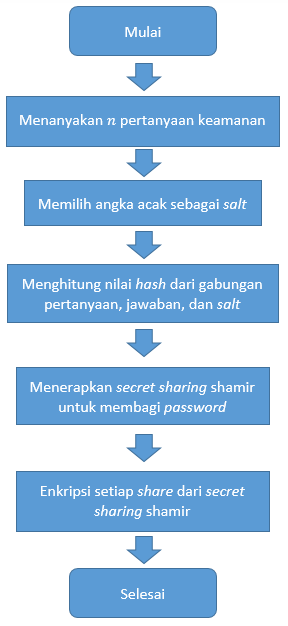
\includegraphics[scale=0.65]{Gambar/flowchart_share}}
	\label{fig:create_share}
	\caption{Proses pembangunan \textit{share} dari \textit{password}}
\end{figure}

Kemudian, untuk alur proses pembangunan kembali atau rekonstruksi \textit{password} dari \textit{share-share} yang adalah sebagai berikut.

%diagram
\begin{figure}[H]
	\centerline{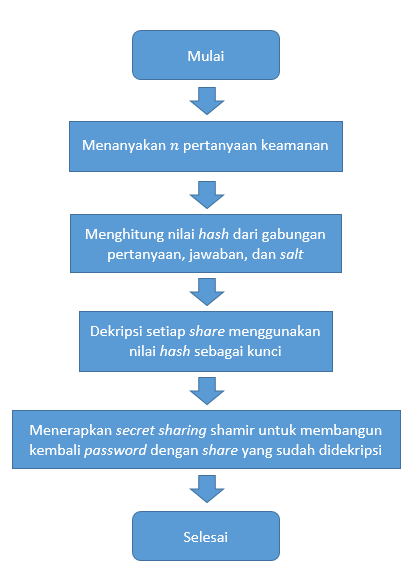
\includegraphics[scale=0.65]{Gambar/flowchart_reconstruct}}
	\label{fig:reconstruct_secret}
	\caption{Proses pembangunan kembali atau rekonstruksi \textit{password}}
\end{figure}

\subsection{Diagram \textit{Use Case}}

Perangkat lunak yang dibangun akan memiliki 2 fitur utama, yaitu menyimpan \textit{password} beserta pertanyaan keamanan yang sifatnya personal dan mengembalikan \textit{password}. Saat menyimpan \textit{password}, pengguna akan diminta untuk menambahkan pertanyaan keamanan yang sifatnya personal dan saat mengembalikan \textit{password}, pengguna akan diminta untuk menjawab pertanyaan keamanan yang sudah disimpan saat menyimpan \textit{password}. Diagram \textit{use case} di bawah ini menunjukkan kedua fitur utama.

%diagram
\begin{figure}[H]
	\centerline{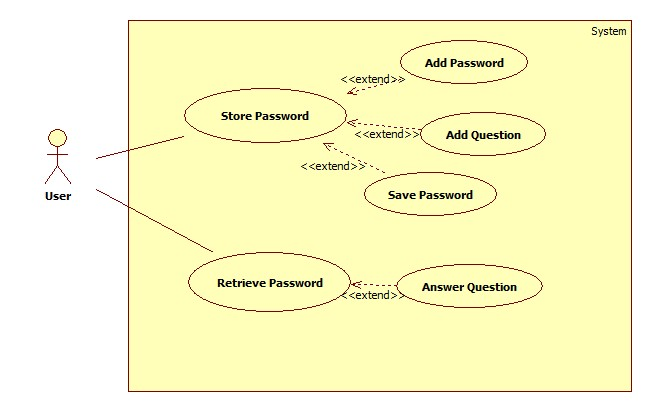
\includegraphics[scale=0.4]{Gambar/use_case}}
	\label{fig:use_case}
	\caption{Diagram \textit{use case} dari perangkat lunak}
\end{figure}

\subsection{Diagram Aktivitas}

Perangkat lunak yang dibangun memiliki 2 proses, yaitu menyimpan \textit{password} atau \textit{secret} dan mengembalikan \textit{password} atau \textit{secret}. Diagram aktivitas di bawah ini menunjukkan proses menyimpan \textit{password} atau \textit{secret}.

%diagram
\begin{figure}[H]
	\centerline{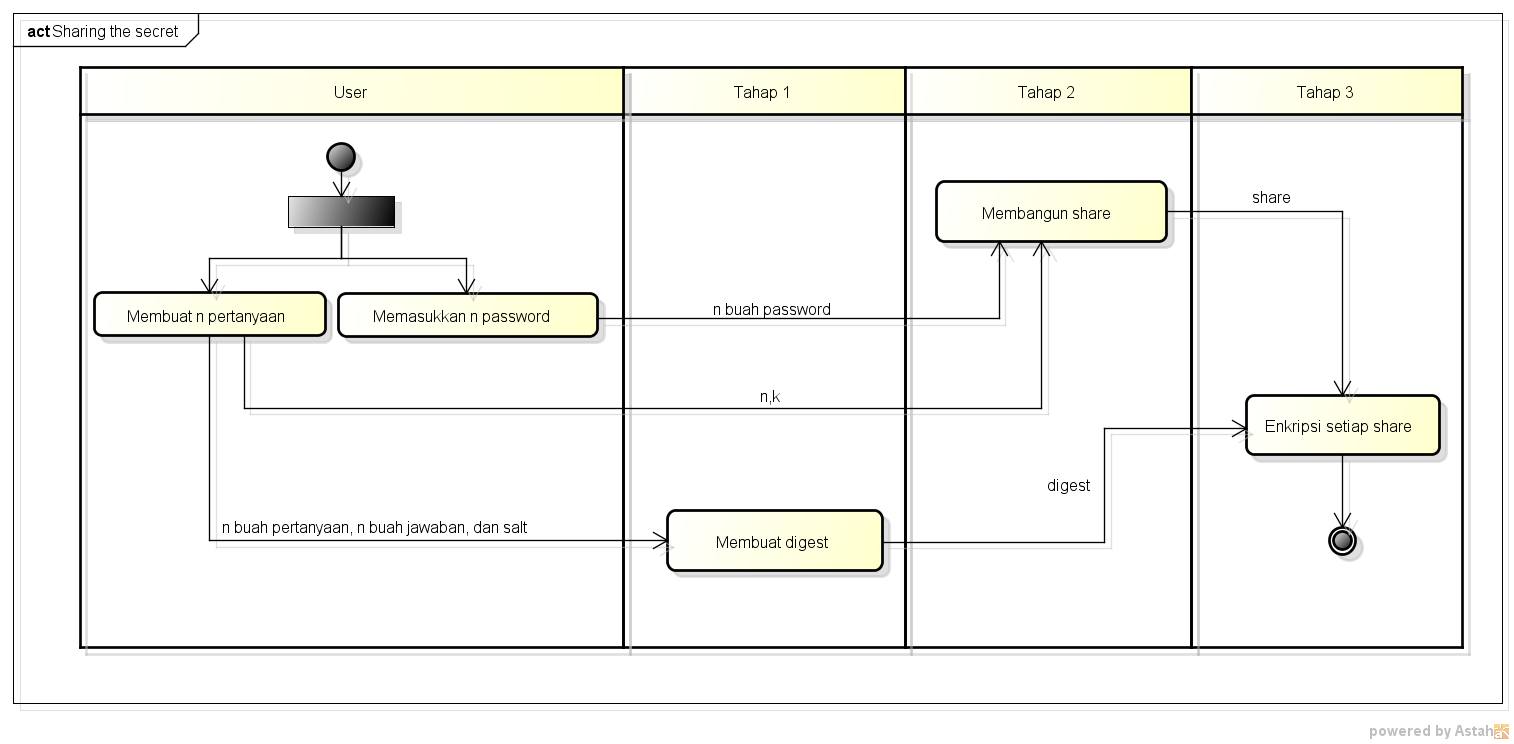
\includegraphics[scale=0.4]{Gambar/sharing-secret}}
	\label{fig:sharing-secret}
	\caption{Diagram aktivitas untuk menyimpan \textit{password}}
\end{figure}

Dalam proses menyimpan \textit{password}, awalnya \textit{user} harus terlebih dahulu menentukan banyak pertanyaan keamanan yang hendak digunakan (\begin{math}n\end{math}) dan banyak minimal pertanyaan keamanan yang bisa dijawab dengan benar untuk memeperoleh kembali \textit{password} (\begin{math}k\end{math}). Kemudian, \textit{user} akan menentukan pertanyaan keamanan personal yang akan digunakan.

Pertanyaan keamanan ini nantinya akan kembali digunakan untuk memperoleh kembali \textit{password} yang hilang atau dilupakan. Kemudian, setelah \textit{user} memilih dan menjawab setiap pertanyaan keamanan, setiap pertanyaan keamanan ini akan dihitung nilai \textit{hash}nya. Selanjutnya dengan menggunakan skema \textit{threshold (k, n)} untuk membagi \textit{password} menjadi sebanyak \begin{math}n\end{math} \textit{share}. Setiap \textit{share} ini akan dienkripsi dengan kunci nilai \textit{hash}.

Selanjutnya adalah proses untuk mengembalikan \textit{password}. Gambar \ref{fig:reconstruct} menunjukkan proses mengembalikan \textit{password}.

%diagram
\begin{figure}[H]
	\centerline{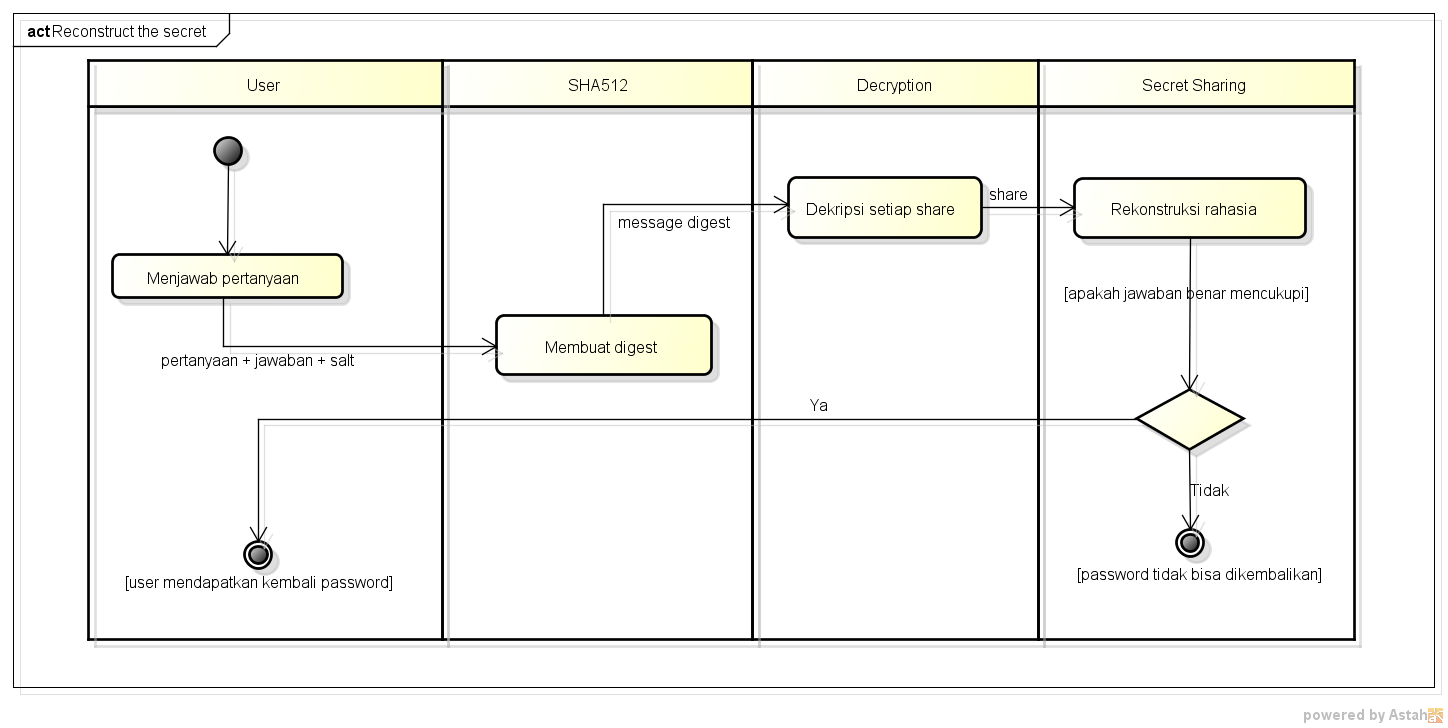
\includegraphics[scale=0.4]{Gambar/reconstruct-secret}}
	\caption{Diagram aktivitas untuk mengembalikan \textit{password}}\label{fig:reconstruct}
\end{figure}

Dalam proses untuk mengembalikan \textit{password}, \textit{user} akan diminta untuk menjawab beberapa pertanyaan keamanan yang sudah dipilih saat \textit{user} menyimpan \textit{password}. Selanjutnya adalah proses yang sama saat meyimpan \textit{password}, yaitu menghitung nilai \textit{hash} dari pertanyaan kemanan yang sudah dijawab oleh \textit{user}. Langkah selanjutnya adalah mendekripsi setiap \textit{share} dengan menggunakan kunci nilai \textit{hash}.

Langkah selanjutnya adalah dengan menggunakan skema \textit{threshold (k, n)} membangun atau rekontruksi ulang \textit{password}. Jika banyak pertanyaan yang dijawab benar oleh \textit{user} sama dengan atau lebih dari \begin{math}k\end{math} \textit{share}, maka \textit{user} bisa mendapatkan kembali \textit{password}, dan jika kurang dari \begin{math}k\end{math} \textit{share} maka \textit{user} tidak bisa mendapatkan kembali \textit{password}.

\subsection{Diagram Kelas}

Perangkat lunak yang dibangun memiliki 2 bagian utama, yaitu bagian \textit{engine} dan bagian antarmuka (\textit{user interface}). Bagian \textit{engine} berfungsi untuk menyimpan dan mengembalikan \textit{password}, melakukan proses enkripsi dan dekripsi, dan melakukan \textit{secret sharing}.

Bagian \textit{engine} merupakan sekumpulan kelas \textit{Java}, sedangkan bagian \textit{antarmuka} akan terdiri dari sekumpulan \textit{Java Server Page} atau JSP. Pada bagian ini akan dijelaskan bagian \textit{engine} saja.

%diagram
\begin{figure}[H]
	\centerline{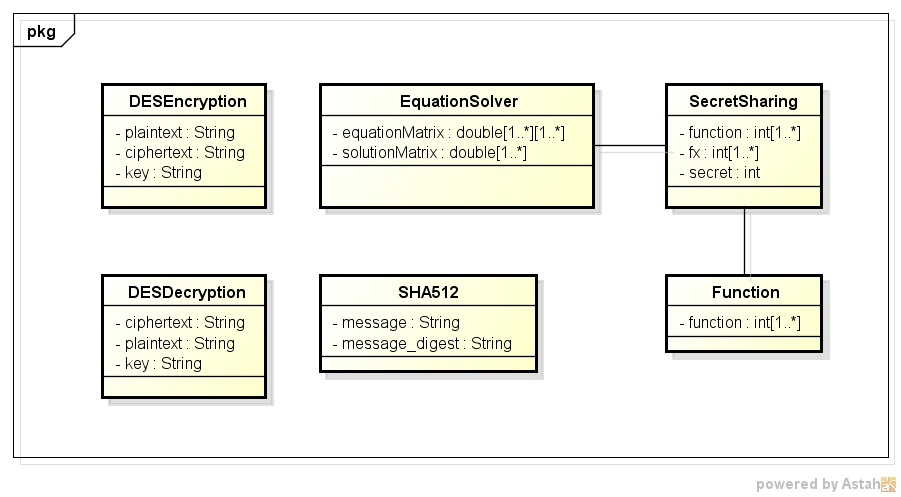
\includegraphics[scale=0.6]{Gambar/engine-class-diagram}}
	\label{fig:reconstruct-secret}
	\caption{Diagram kelas \textit{engine}}
\end{figure}

Untuk proses penyimpanan \textit{password}, kelas SHA512 berfungsi untuk menghitung nilai \textit{hash} dari gabungan pertanyaan, jawaban, dan \textit{salt}. Selanjutnya, kelas SecretSharing akan membagi \textit{password} menjadi beberapa \textit{share}. Kemudian, kelas DESEncryption akan mengenkripsi setiap \textit{share} dengan nilai \textit{hash} sebagai kunci rahasia. Setiap \textit{ciphertext} hasil enkripsi, nilai \textit{salt}, dan pertanyaan akan disimpan.

Untuk proses pengembalian \textit{password}, kelas SHA512 akan menghitung nilai \textit{hash} dari gabungan pertanyaan, jawaban, dan \textit{salt}. Kemudian, kelas DESDecryption akan mendekripsi \textit{ciphertext} hasil enkripsi yang disimpan dan kunci rahasia dari nilai \textit{hash} untuk memperoleh \textit{plaintext}. Kelas SecretSharing akan merekontruksi \textit{password} berdasarkan hasil dekripsi dari kelas DESDecryption. Jika, banyak pertanyaan benar sesuai, maka \textit{password} bisa dikembalikan.

\subsection{Arsitektur Perangkat Lunak}

Pada bagian sebelumnya sudah dijelaskan mengenai alur proses, diagram \textit{use case}, diagram aktivitas, dan diagram kelas dari perangkat lunak yang dibangun. Pada bagian ini akan dijelaskan mengenai seluruh bagian perangkat lunak yang dibangun. Seperti yang sudah dijelaskan sebelumnya perangkat lunak yang dibangun memiliki 2 bagian utama, yaitu bagian \textit{engine} dan bagian antarmuka.

%diagram
\begin{figure}[H]
	\centerline{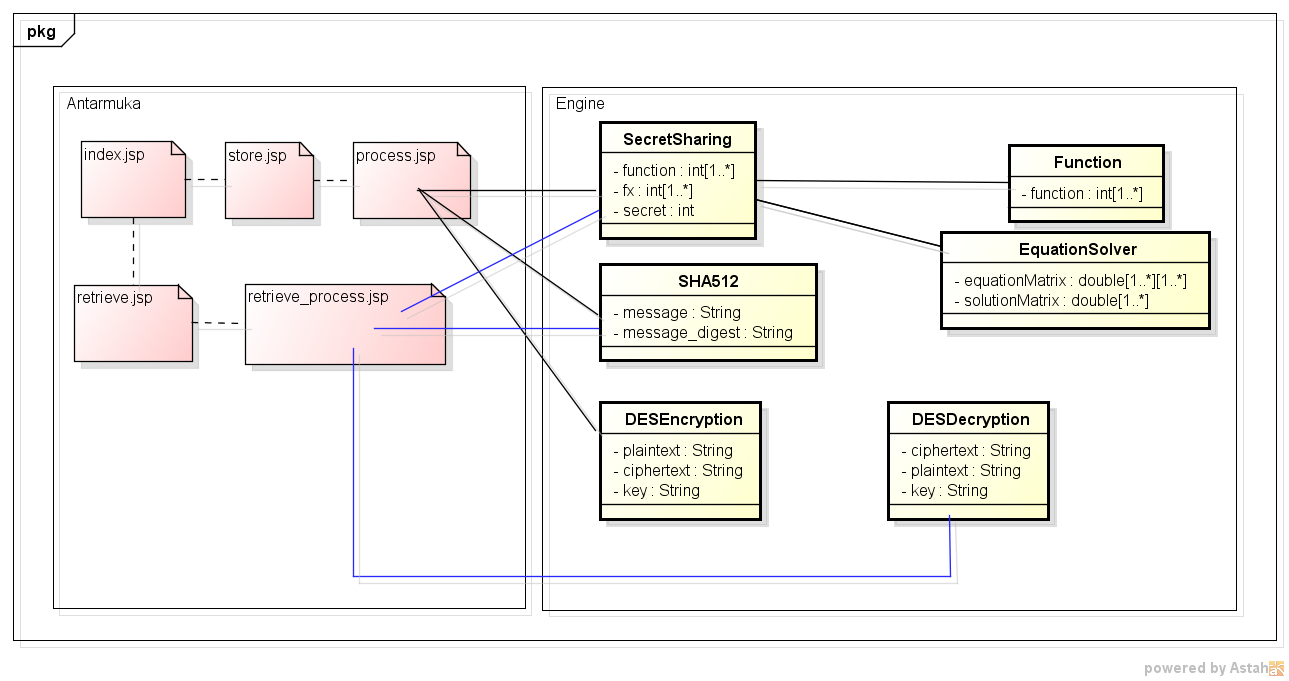
\includegraphics[scale=0.5]{Gambar/arsitektur}}
	\label{fig:arsitektur-perangkat-lunak}
	\caption{Arsitektur perangkat lunak}
\end{figure}

Untuk proses penyimpanan \textit{password}, sama seperti pada bagian sebelumnya, kelas yang akan digunakan adalah kelas SHA512 untuk menghasilkan \textit{hash}, kemudian kelas SecretSharing untuk menghasilkan \textit{share} dari \textit{password}, dan kelas DESEncryption untuk mengenkripsi masing-masing dari \textit{share} dengan nilai \textit{hash} sebagai kunci rahasia.

Selanjutnya, untuk proses pengembalian \textit{password}, kelas SHA512 akan digunakan kembali untuk menghasilkan \textit{digest}. Setelah \textit{digest} dihasilkan, kelas DESDecryption akan mendekripsi \textit{share-share} yang dimiliki dengan kunci \textit{digest} yang dihasilkan. Selanjutnya, kelas SecretSharing akan merekonstruksi ulang hasil dekripsi dari kelas DESDecryption dan menentukan apakah \textit{password} bisa dikembalikan atau tidak.